\documentclass[11pt]{article}
\usepackage{classTools}


\begin{document}



% To include a problems set header, use the psHeader command
\psHeader{3}{Wed Sept. 28, 2022 (11:59pm)}

\textbf{Your name: }

\textbf{Collaborators: }

\textbf{No. of late days used on previous psets: }

\textbf{No. of late days used after including this pset: }


The purpose of this problem set is to solidify your understanding of the RAM model (and variants), and the relations between the RAM model, the Word-RAM model, Python programs, and variants. In particular, you will build skills in simulating one computational model by another and in evaluating the runtime of the simulations (both in theory and in practice).

\begin{enumerate}
 
    \item (Simulation in practice: RAMs on Python)  
    In the Github repository, we have given you a partially written Python implementation of a RAM Model simulator.  Your task is to fill in the missing parts of the code to obtain a complete RAM simulator.
     Your simulator should take as input a RAM Program $P$ and an input $x$, and simulate the execution of $P$ on $x$, and return whatever output $P$ produces (if it halts).  The RAM Program $P$ is given as a Python list $[v,C_0,C_1,\ldots,C_{\ell-1}]$, where $v$ is the number of variables used by $P$.  For simplicity, we assume that the variables are named $0,\ldots,v-1$ (rather than having names like ``tmpptr'' and ``insertvalue''), but you can introduce constants to give names to the variables.  The $0$\textsuperscript{th} variable will always be $\inputlen$, the $1$\textsuperscript{st} variable $\outputpointer$, and the $2$\textsuperscript{nd} variable $\outputlen$.  A command $C$ is given in the form of a list of the form $[\cmd]$, $[\cmd,i]$, $[\cmd,i,j]$, or $[\cmd,i,j,k]$, where $\cmd$ is the name of the command and $i,j,k$ are the indices of the variables or line numbers used in the command.  For example,  the command $\var_i = M[\var_j]$ would be represented as $(\READ,i,j)$.  See the Github repository for the precise syntax as well as some RAM programs you can use to test your simulator.

    \item (Empirically evaluating simulation runtimes and explaining them theoretically)  


Consider the following two RAM programs:

\begin{algorithm}[H]
\Input{A single natural number $N$ (as an array of length 1)}
\Output{$11^{2^N+1}$ (as an array of length 1)}
\Variables{$\inputlen, \outputpointer, \outputlen, \counter, \result$}
\setcounter{AlgoLine}{-1}
$\zero = 0$\;
$\one = 1$\;
$\eleven = 11$\;
$\outputlen = 1$\;
$\outputpointer = 0$\;
$\result = 11$\;
$\counter = M[\zero]$\;
\Indp
 IF $\counter == 0$ GOTO 11\;
$\result = \result * \result$\;
$\counter = \counter - \one$\;
IF $\zero == 0$ GOTO 7\;
\Indm
$\result = \result * \eleven$\; \label{line:done}
$M[\outputpointer]=\result$\;
\end{algorithm}


\begin{algorithm}[H]
\Input{A single natural number $N$ (as an array of length 1)}
\Output{$11^{2^N+1} \bmod 2^{32}$ (as an array of length 1)}
\Variables{$\inputlen, \outputpointer, \outputlen, \counter, \result, \temp, \W$}
\setcounter{AlgoLine}{-1}
$\zero = 0$\;
$\one = 1$\;
$\eleven = 11$\;
$\outputlen = 1$\;
$\outputpointer = 0$\;
$\result = 11$\;
$\W = 2^{32}$\;
$\counter = M[\zero]$\;
\Indp
IF $\counter == 0$ GOTO 15 \;
$\result = \result * \result$\;
$\temp = \result / \W$\;
$\temp = \temp \times \W$\;
$\result = \result - \temp$\;
$\counter = \counter - \one$\;
IF $\zero == 0$ GOTO 8 \;
\Indm
$\result = \result * \eleven$\;
\label{line:done2}
$\temp = \result / \W$\;
$\temp = \temp \times \W$\;
$\result = \result - \temp$\;
$M[\outputpointer]=\result$\; 
\end{algorithm}


\begin{enumerate}
    \item \label{itm:RAMtime} Exactly calculate (without asymptotic notation) the RAM-model running times of the above algorithms as a function of $N$.
    Which one is faster? 

\begin{proof}

\end{proof}
    
    \item \label{itm:realtime} Using your RAM Simulator, run both RAM programs on inputs $N=0,1,2,\ldots,15$ and graph the actual running times (in clock time, not RAM steps).  (We have provided you with some timing and graphing code in the Github repository.) Which one is faster? 
    
\begin{proof}[Solution]
Here is the plot.
\\
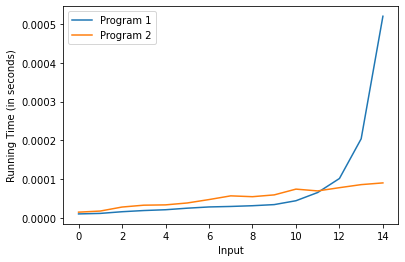
\includegraphics[width=5in]{2-2}

It looks like the first program is slightly faster until $N = 12$, at which point it becomes dramatically slower than the second program.
\end{proof}  
    
    \item Explain the discrepancies you see between Parts~\ref{itm:RAMtime} and \ref{itm:realtime}.  (Hint: What do we know about the relationship between the RAM and Word-RAM models, and why is it relevant to how efficiently the Python simulation runs?)  
    
    \item (optional\footnote{This problem won't make a difference between N, L, R-, and R grades.}) Give a theoretical explanation (using asymptotic estimates) of the shapes of the runtime curves you see in Part~\ref{itm:realtime}. You may need to do some research online and/or make guesses about how Python operations are implemented to come up with your estimates. 

\end{enumerate}

\item (Simulating Word-RAM by RAM)  Show that for every Word-RAM program $P$, there is a RAM program $P'$ such that $P'$ halts on $x$ iff $P$ halts on $x$, and if they halt, then  $P'(x)=P(x)$ and 
       $$\Time_{P'}(x) = O\left(\Time_P(x)+n+w_0\right),$$
where $n$ is the length of $x$ and $w_0$ is the initial word size of $P$ on input $x$.  (This was stated without proof in Lecture Notes 7.) 

Your proof should use an {\em implementation-level} description, similar to our proof that RAM programs can be simulated by ones with at most $c$ registers.  Recall that Word-RAM programs have read-only variables $\memsize$ and $\wordlen$; you may want to start your simulation by calculating these variables as well as another variable representing $2^{\wordlen}$.  Then think about how each operation of a Word-RAM program $P$ can be simulated in a RAM program $P'$, taking care of any differences between their semantics in the Word-RAM model vs. the RAM model. Don't forget MALLOC!

\end{enumerate}


\end{document}
